\section{Create image}
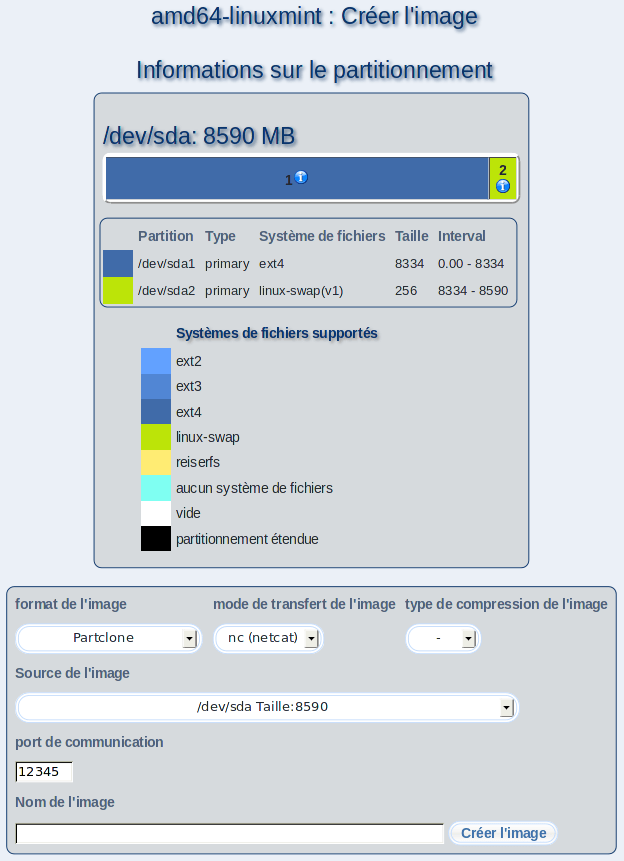
\includegraphics[scale=0.4]{/mdk/doc/manual/screenshots/en/client_createImage.png} \\
You can create images from a partition or a whole drive of your client in this dialog. This image can be used to install clients. Select your preferred Image format, the Image transfer type and the Image compression. You have to make additional designations under \textit{"Image source"} for some image formats e.g. the partition or drive that should be stored in the image.\\
Choose a name for the image and enter it at \textit{"Image name"}. Click on \textit{"Create image"} afterwards.\\
\subsection{Hint for image files}
The files are stored in the directory \textbf{/m23/data+scripts/clientImages} in different types and with distinct compressions. The file names are always created after the following scheme: $\langle$Image name$\rangle$$\langle$Size of the extracted image in bytes$\rangle$$\langle$Image format$\rangle$$\langle$Compression$\rangle$\\
Image format is one of the following values:\\
\begin{itemize}
\item \textbf{dd}: Saves the whole data of a partition or harddisk.\\
\end{itemize}
For the compression the following is valid:\\
\begin{itemize}
\item (no extension): The image file will be stored with no compression.\\
\item \textbf{gz}: The image will be compressed with  gzip.\\
\item \textbf{bz2}: It will be compressed with bzip2 that compresses better mostly.\\
\end{itemize}
\subsection{Hint for the Transfer port}
You have to enter a network port that can be used on client and server side and is not blocked (e.g. firewall) for the Image transfer type. If you want to create images from multiple clients concurrently you have to choose different port numbers.\\
